% ============================================================
% Corrigé du TP : La loi normale au service du contrôle de fabrication -- butée
% Pôle Formation UIMM - CVDL - BTS CPRP - S. JAUBERT
% Énoncé : MOD08_TP_CPRP_Capabilite_Butee_v2_0
% ============================================================
\documentclass[a4paper,11pt]{article}
% Préambule commun TP / corrigé -- MOD08 TP CPRP capabilité d'une butée
\usepackage[utf8]{inputenc}
\usepackage[T1]{fontenc}
% babel-french absent sur certains postes : chargement conditionnel
\IfFileExists{french.ldf}{\usepackage[french]{babel}}{}
\usepackage{helvet}
\usepackage{courier}
\renewcommand{\familydefault}{\sfdefault}
\usepackage[top=3cm, bottom=2.5cm, left=2cm, right=2cm, headheight=2cm]{geometry}
\usepackage{amsmath,amssymb,amsfonts}
\usepackage{graphicx}
\usepackage[dvipsnames,table]{xcolor}
\usepackage{tikz}
\usepackage{pgfplots}
\pgfplotsset{compat=1.16}
\usepackage[most]{tcolorbox}
\usepackage{fancyhdr}
\usepackage{enumitem}
\usepackage{array,needspace,booktabs}
\usepackage{titlesec}
\usepackage{hyperref}

\definecolor{uimmblue}{HTML}{005C85}
\definecolor{uimmred}{HTML}{D31326}
\definecolor{uimmlightblue}{HTML}{E8F1F8}
\definecolor{uimmgray}{HTML}{333333}
\definecolor{uimmlightgray}{HTML}{F5F5F5}
\definecolor{ctlgreen}{HTML}{2E8B3D}
\hypersetup{colorlinks=true, linkcolor=uimmblue, urlcolor=uimmblue}

\titleformat{\section}{\Large\bfseries\color{uimmblue}}{}{0pt}{}[\vspace{2pt}{\color{uimmblue}\titlerule[1.2pt]}]
\titleformat{\subsection}{\large\bfseries\color{uimmblue}}{}{0pt}{}
\setlist[enumerate,1]{label={\color{uimmblue}\textbf{\arabic*.}}, leftmargin=*}
\setlist[enumerate,2]{label=\alph*), leftmargin=*}
\setlist[itemize,1]{label={\color{uimmblue}\textbullet}}

\newtcolorbox{exo}[1]{colback=white, colframe=uimmblue, fonttitle=\bfseries\color{white},
  coltitle=white, title={#1}, boxrule=1pt, arc=2pt,
  left=8pt, right=8pt, top=5pt, bottom=6pt, before skip=10pt, after skip=6pt}
\newtcolorbox{consigne}{colback=uimmlightgray, colframe=uimmgray, boxrule=0.8pt, arc=3pt,
  left=8pt, right=8pt, top=6pt, bottom=6pt}
\newtcolorbox{rappel}[1]{colback=uimmlightblue, colframe=uimmblue, fonttitle=\bfseries\color{white},
  coltitle=white, title={#1}, boxrule=0.8pt, arc=2pt,
  left=8pt, right=8pt, top=4pt, bottom=4pt, before skip=7pt, after skip=6pt}

\newcommand{\calc}{\,{\color{uimmred}\small\textbf{[calculatrice]}}}
\newcommand{\tabl}{\,{\color{uimmred}\small\textbf{[Excel]}}}
\newcommand{\xl}{\,{\color{uimmred}\small\textbf{[Excel]}}}
\newcommand{\duree}[1]{\hfill{\normalsize\color{uimmred}#1}}
\newcommand{\Dbar}{\overline{D}}
\newcommand{\Dbb}{\overline{\overline{D}}}
\newcommand{\Rbar}{\overline{R}}
% Zone de réponse lignée : #1 = nombre de lignes
\newcommand{\zone}[1]{\par\smallskip\noindent\begin{tikzpicture}
  \foreach \i in {1,...,#1}{\draw[uimmgray!30] (0,-0.74*\i) -- (\linewidth-1pt,-0.74*\i);}
  \end{tikzpicture}\par\smallskip}
\newcommand{\EnTete}[1]{%
\pagestyle{fancy}\fancyhf{}\renewcommand{\headrulewidth}{0pt}
\fancyhead[L]{\raisebox{-0.5\height}{
\includegraphics[height=1.5cm]{logo_uimm_placeholder.jpg}}}
\fancyhead[C]{\begin{minipage}{8cm}\centering
  {\small\color{uimmblue}\textbf{Pôle Formation UIMM - CVDL}}\\
  {\footnotesize\color{uimmgray} BTS CPRP -- Mathématiques}\end{minipage}}
\fancyhead[R]{{\small\color{uimmblue}\textbf{MOD08 -- #1}}}
\fancyfoot[C]{{\color{uimmblue}\rule{\textwidth}{1pt}}\\[2pt]
  {\footnotesize\color{uimmgray} Pôle Formation UIMM -- Centre-Val de Loire \hfill S. JAUBERT \hfill \thepage}}}
% Cartes de contrôle vierges (dossier réponse) : #1 = légende y, ymin, ymax, pas
\pgfplotsset{ctl/.style={width=0.93\linewidth, height=6.3cm, xmin=0.5, xmax=10.5, xtick={1,2,3,4,5,6,7,8,9,10},
  grid=both, minor y tick num=4, grid style={uimmgray!35}, minor grid style={uimmgray!15},
  xlabel={Numéro de l'échantillon}, tick label style={font=\footnotesize},
  /pgf/number format/use comma, /pgf/number format/fixed, /pgf/number format/precision=3,
  /pgf/number format/fixed zerofill, scaled y ticks=false,
  xticklabel={\pgfmathprintnumber[fixed,precision=0]{\tick}}}}
\EnTete{Corrigé TP}
\newtcolorbox{correction}[1][]{%
  colback=green!5, colframe=green!50!black,
  fonttitle=\bfseries\color{white}, title={\textsf{Correction}~#1},
  coltitle=white, boxrule=1pt, arc=3pt,
  left=8pt, right=8pt, top=6pt, bottom=6pt, before skip=8pt, after skip=8pt, breakable}
\newcommand{\source}[1]{{\footnotesize\color{uimmgray}\textbf{Réf.}\enspace #1}\par\smallskip}
\newcommand{\piege}[1]{\par\smallskip{\footnotesize\color{uimmred!80!black}\textbf{Erreurs attendues~:} #1}}
\newcommand{\xlf}[1]{\par\smallskip{\footnotesize\color{uimmgray}\textbf{Excel}\enspace #1}}
\newcommand{\LN}{Cours MOD08 \textit{Loi normale}}
\newcommand{\LD}{Cours MOD08 \textit{Lois discrètes}}
\newcommand{\DR}{TP, dossier de référence pp.~2--3}
\newcommand{\TDv}{TD v2, encadré \textit{Outils mobilisés} p.~1}

\begin{document}

\begin{tcolorbox}[colback=uimmblue, colframe=uimmblue, sharp corners, boxrule=0pt,
  left=14pt, right=14pt, top=8pt, bottom=8pt]
{\color{white}\LARGE\bfseries Corrigé -- TP MOD08}\\[4pt]
{\color{white}\large La loi normale au service du contrôle de fabrication \hfill Document formateur}\\[2pt]
{\color{white}\normalsize Cartes de contrôle et capabilité du diamètre d'une butée}
\end{tcolorbox}

\begin{consigne}\footnotesize
\textbf{Repères d'animation.}
\begin{itemize}[leftmargin=12pt, itemsep=1pt, topsep=2pt]
  \item \textbf{Objectif}~: montrer que la loi normale sert, en métrologie et en méthodes, à fixer les limites des cartes de contrôle, à prévoir la proportion de pièces hors tolérance et à régler un procédé (cartes, $C_p$, $C_{pk}$, fenêtre de réglage).
  \item \textbf{Durées}~: A 25 min (dont la mesure des échantillons $7$ à $10$), B 40 min, C 30 min, D 15 min, soit 110 min. Les questions B.7 et D.2 se retirent sans casser le fil si le temps manque.
  \item \textbf{Fil rouge}~: les cartes (partie B) révèlent une dérive que la droite de Henry et le $C_{pk}$ global (parties A et C) ne montrent pas. La partie D le chiffre.
  \item \textbf{Fichiers}~: classeur stagiaire (cellules jaunes à compléter, aucune formule) et classeur corrigé (mêmes onglets, formules et graphiques faits). Les valeurs ci-dessous viennent du classeur corrigé, qui contient les échantillons $7$ à $10$ de référence.
  \item \textbf{Les stagiaires mesurent leurs propres échantillons $7$ à $10$}~: leurs résultats seront proches des vôtres, pas identiques. Ne dépendent \emph{pas} des mesures~: $z_c$, $z_s$, les coefficients, B.7, C.3, $\sigma_{\max}$ de C.5, la loi binomiale de B.6. Dépendent des mesures~: moyennes, étendues, $\sigma$, limites, $C_p$, $C_{pk}$, fenêtre de réglage, $s$, pente. Accepter tout résultat cohérent avec les données du stagiaire~; vérifier la \emph{méthode}.
  \item \textbf{Deux points de bascule}~: avec le jeu de référence, la moyenne de l'échantillon $8$ ($11{,}9352$) dépasse $LCS$ ($11{,}9347$) de $0{,}5$ \textmu m, et l'étendue $R_6 = 0{,}080$ dépasse $LS_2$ ($0{,}0796$) de $0{,}4$ \textmu m. Selon les mesures et les arrondis, ces deux points peuvent basculer~: demander une justification, ne pas imposer le résultat.
  \item \textbf{Fonctions Excel (version française)}~: voir §5 du dossier de référence. Les anciens noms (\texttt{LOI.NORMALE}, \texttt{LOI.NORMALE.\allowbreak STANDARD.\allowbreak INVERSE}, \texttt{ECARTYPE}) restent valables. Les formules attendues sont dans le classeur corrigé, onglet Calculs, colonne B.
  \item \textbf{Points d'attention}~: (1) $50$ mesures, c'est peu~: le dossier rappelle $100$ à $200$ relevés. (2) Les échantillons $1$ à $6$ sont au centième, les échantillons $7$ à $10$ de référence au millième~: résolution mélangée, sans effet sur la méthode. (3) Les limites sont calculées avec des données qui contiennent la dérive~: c'est une première étude, pas une carte de suivi. (4) Dans le tableau de l'ancien TP, $D_{c2}$ pour $n = 5$ est écrit $5{,}58$~; la valeur correcte est $5{,}48$. Ce coefficient n'est pas utilisé ici.
  \item \textbf{Références}~: \DR{} et sections du \LN{} ou du \LD{} (pagination imprimée en pied de page).
  \item \textbf{Contrôle}~: toutes les valeurs ont été recalculées indépendamment en Python (\texttt{scipy.stats}) et dans le classeur (LibreOffice), sans écart.
\end{itemize}
\end{consigne}

\begin{center}\footnotesize
\renewcommand{\arraystretch}{1.15}
\begin{tabular}{llll}
\toprule
\textbf{Partie} & \textbf{Question} & \textbf{Savoir-faire} & \textbf{Résultat de référence} \\
\midrule
A & A.2 & $\sigma = \Rbar/d_n$ & $\sigma = 18{,}9$ \textmu m \\
A & A.4 & droite de Henry & points alignés, normalité plausible \\
B & B.2 & seuils $z_c$, $z_s$ & $z_c = 3{,}09$, $z_s = 1{,}96$ \\
B & B.5 & lecture des cartes & dérive vers le haut, $5$ points hors $LC$ \\
B & B.6 & fausse alerte & $P(X \geq 1) \approx 0{,}0198$ \\
C & C.2 & $C_p$, $C_{pk}$ & $1{,}32$ et $1{,}03$ \\
C & C.4 & fenêtre de réglage & $[11{,}921\,;11{,}929]$, réglage hors fenêtre \\
C & C.5 & $\sigma_{\max}$ & $18{,}4$ \textmu m, donc non tenu \\
D & D.1 & indices sur la durée & $C_{pk} \approx 0{,}54$ \\
D & D.2 & prévision contre réalité & $978$ ppm prévus, $40\,000$ ppm observés \\
\bottomrule
\end{tabular}
\end{center}

% ============================================================
\newpage
\section{Partie A -- Décrire le procédé}

\needspace{7cm}
\begin{correction}[-- A.1]
\source{\DR{}, §1}
\begin{center}\footnotesize
\renewcommand{\arraystretch}{1.2}
\begin{tabular}{|l|*{10}{c|}}\hline
Échantillon $i$ & 1 & 2 & 3 & 4 & 5 & 6 & 7 & 8 & 9 & 10 \\ \hline
$\Dbar_i$ (mm) & $11{,}864$ & $11{,}862$ & $11{,}884$ & $11{,}898$ & $11{,}910$ & $11{,}902$ & $11{,}928$ & $11{,}935$ & $11{,}942$ & $11{,}960$ \\ \hline
$R_i$ (mm) & $0{,}040$ & $0{,}050$ & $0{,}050$ & $0{,}040$ & $0{,}040$ & $0{,}080$ & $0{,}050$ & $0{,}026$ & $0{,}024$ & $0{,}040$ \\ \hline
\end{tabular}
\end{center}
\[
\begin{gathered}
\Dbb = \frac{1}{10}\sum_{i=1}^{10}\Dbar_i = 11{,}9086 \text{ mm},\\[4pt]
\Rbar = \frac{1}{10}\sum_{i=1}^{10}R_i = 0{,}044 \text{ mm}.
\end{gathered}
\]
\xlf{\texttt{=MOYENNE(B2:F2)} et \texttt{=MAX(B2:F2)-MIN(B2:F2)}, recopiées vers le bas~; puis \texttt{=MOYENNE(G2:G11)} et \texttt{=MOYENNE(H2:H11)}.}
\piege{prendre l'écart-type de l'échantillon à la place de l'étendue~; calculer l'étendue entre deux mesures consécutives~; oublier l'échantillon $10$ dans la moyenne (plage trop courte).}
\end{correction}

\needspace{5cm}
\begin{correction}[-- A.2]
\source{\DR{}, §1~; \LN{}, §3.1 Rôle des paramètres p.~6}
\[
\sigma = \frac{\Rbar}{d_5} = \frac{0{,}044}{2{,}326} \approx 0{,}0189 \text{ mm} = 18{,}9 \text{ \textmu m}.
\]
On retient $D \sim \mathcal{N}(11{,}9086\,;0{,}0189)$.
\piege{prendre $\sigma = \Rbar = 44$ \textmu m~; oublier de diviser par $d_n$~; confondre mm et \textmu m.}
\end{correction}

\needspace{6cm}
\begin{correction}[-- A.3]
\source{\LN{}, §3.4 La règle des 68 -- 95 -- 99,7 p.~7}
\begin{enumerate}
  \item $3\sigma = 56{,}7$ \textmu m, donc $[11{,}9086 - 0{,}0567\,;11{,}9086 + 0{,}0567] = [11{,}852\,;11{,}965]$. Cet intervalle contient environ $99{,}7\,\%$ des pièces.
  \item Il est dans la tolérance $[11{,}85\,;12{,}00]$, mais il touche presque la borne basse. Marge côté bas~: $11{,}852 - 11{,}850 = 2$ \textmu m. Marge côté haut~: $12{,}000 - 11{,}965 = 35$ \textmu m. L'intervalle est large ($6\sigma = 113{,}5$ \textmu m pour $IT = 150$ \textmu m) et décentré vers la borne basse. C'est le point de départ de $C_p$ et $C_{pk}$ (partie C).
\end{enumerate}
\piege{confondre l'intervalle de dispersion du procédé avec l'intervalle de tolérance.}
\end{correction}

\needspace{9cm}
\begin{correction}[-- A.4]
\source{\LN{}, §2.3 Problème inverse p.~5~; \DR{}, §1 (la relation $\sigma = \Rbar/d_n$ suppose une loi normale) et §5 (Excel)}
Les rangs vont de $1$ à $50$~; $p_k = (k - 0{,}5)/50$, donc $z_k$ va de $-2{,}326$ ($k = 1$) à $+2{,}326$ ($k = 50$).

\smallskip
\textbf{Lecture.} Les points sont proches de la droite, sur toute la plage des valeurs (coefficient de corrélation $0{,}988$). Quelques marches apparaissent, à cause des valeurs égales relevées au centième dans les échantillons $1$ à $6$. Les deux mesures de $11{,}84$ sont légèrement sous la droite, ce qui est sans gravité.

\smallskip
\textbf{Conclusion attendue.} La distribution des $50$ mesures prises ensemble paraît normale. On garde le modèle $D \sim \mathcal{N}(\mu\,;\sigma)$. \emph{Attention, c'est un piège pédagogique~:} la droite de Henry ne dit rien de l'ordre des mesures. Un procédé qui dérive peut produire un ensemble de valeurs d'allure normale. Les cartes (partie B) montrent ce que la droite de Henry ne voit pas, et la partie D y revient. Remarque formateur~: avec $50$ valeurs, la droite de Henry reste un outil visuel~; ne pas la transformer en test de normalité.

\xlf{onglet Henry, \texttt{=(A2-0,5)/50}, \texttt{=PETITE.VALEUR(Mesures!\$B\$2:\$F\$11;A2)}, \texttt{=LOI.NORMALE.\allowbreak STANDARD.\allowbreak INVERSE.N(B2)}, puis nuage de points $(d_{(k)}\,;z_k)$.}

\begin{center}
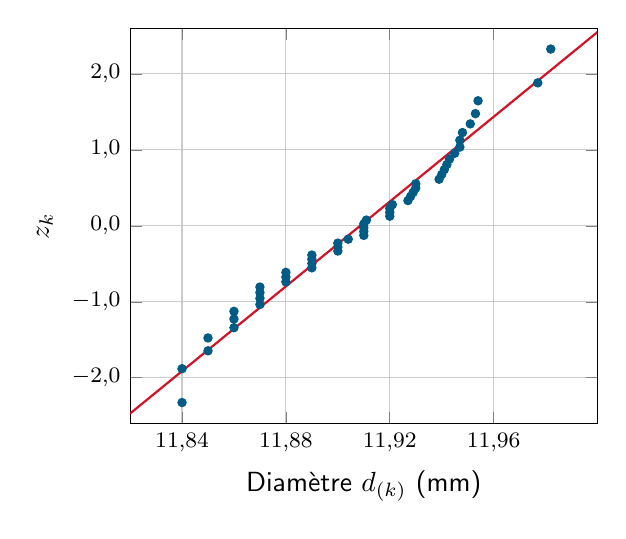
\begin{tikzpicture}
\begin{axis}[width=0.62\linewidth, height=6.6cm, xmin=11.82, xmax=12.00, ymin=-2.6, ymax=2.6, grid=both, grid style={uimmgray!25},
  xlabel={Diamètre $d_{(k)}$ (mm)}, ylabel={$z_k$}, tick label style={font=\footnotesize}, xtick={11.84,11.88,11.92,11.96},
  /pgf/number format/use comma, /pgf/number format/fixed, /pgf/number format/precision=2, /pgf/number format/fixed zerofill,
  xticklabel style={/pgf/number format/precision=2}, yticklabel style={/pgf/number format/precision=1}, scaled ticks=false]
\addplot[only marks, mark=*, mark size=1.5pt, uimmblue] coordinates {(11.840,-2.326) (11.840,-1.881) (11.850,-1.645) (11.850,-1.476) (11.860,-1.341) (11.860,-1.227) (11.860,-1.126) (11.870,-1.036) (11.870,-0.954) (11.870,-0.878) (11.870,-0.806) (11.880,-0.739) (11.880,-0.674) (11.880,-0.613) (11.890,-0.553) (11.890,-0.496) (11.890,-0.440) (11.890,-0.385) (11.900,-0.332) (11.900,-0.279) (11.900,-0.228) (11.904,-0.176) (11.910,-0.126) (11.910,-0.075) (11.910,-0.025) (11.910,0.025) (11.911,0.075) (11.920,0.126) (11.920,0.176) (11.920,0.228) (11.921,0.279) (11.927,0.332) (11.928,0.385) (11.929,0.440) (11.930,0.496) (11.930,0.553) (11.939,0.613) (11.940,0.674) (11.941,0.739) (11.942,0.806) (11.943,0.878) (11.945,0.954) (11.947,1.036) (11.947,1.126) (11.948,1.227) (11.951,1.341) (11.953,1.476) (11.954,1.645) (11.977,1.881) (11.982,2.326)};
\addplot[uimmred, thick, domain=11.82:12.00] {(x-11.90858)/0.035855};
\end{axis}
\end{tikzpicture}

{\footnotesize Droite de Henry des $50$ mesures (points) et droite d'une loi normale de même moyenne et de même écart-type $s$ (trait rouge).}
\end{center}
\piege{conclure «~normal~» sans regarder les extrémités~; conclure «~le procédé est stable~» parce que la droite de Henry est alignée (elle ne regarde pas le temps).}
\end{correction}

% ============================================================
\needspace{8cm}
\section{Partie B -- Cartes de contrôle}

\needspace{5cm}
\begin{correction}[-- B.1]
\source{\LN{}, §6.1 Énoncé p.~12~; \TDv{}~; \DR{}, §2}
\[
\sigma_{\Dbar} = \frac{\sigma}{\sqrt{5}} = \frac{18{,}9}{2{,}236} \approx 8{,}5 \text{ \textmu m}.
\]
Une moyenne de $5$ pièces varie $\sqrt{5} \approx 2{,}2$ fois moins qu'une pièce~: les écarts, dans un sens et dans l'autre, se compensent en partie. C'est ce qui rend la carte des moyennes sensible aux petits décalages.
\piege{utiliser $\sigma$ à la place de $\sigma/\sqrt{5}$~; diviser par $5$ au lieu de $\sqrt{5}$.}
\end{correction}

\needspace{10cm}
\begin{correction}[-- B.2]
\source{\LN{}, §2.3 p.~5 et §4.1 p.~8 (\texttt{FracNormale})~; \DR{}, §2, §4 et §5}
\begin{enumerate}
  \item $P(Z > z_c) = 0{,}001 \iff P(Z \leq z_c) = 0{,}999$, donc $z_c = \texttt{LOI.NORMALE.STANDARD.INVERSE.N(0,999)} \approx 3{,}0902$. De même $P(Z \leq z_s) = 0{,}975$ et $z_s \approx 1{,}9600$.
  \item $\sigma_{\Dbar} = 0{,}0084598$ mm.
  \[
  LCS = 11{,}9086 + 3{,}0902 \times 0{,}0084598 \approx 11{,}935, \qquad LCI = 11{,}9086 - 0{,}026142 \approx 11{,}882,
  \]
  \[
  LSS = 11{,}9086 + 1{,}9600 \times 0{,}0084598 \approx 11{,}925, \qquad LSI = 11{,}9086 - 0{,}016581 \approx 11{,}892.
  \]
  \item $z_c/\sqrt{5} \approx 1{,}3820 = A_c$ et $z_s/\sqrt{5} \approx 0{,}8765$, contre $A_s = 0{,}876$ dans le tableau (écart d'arrondi). Les coefficients du tableau ne sont donc pas magiques~: ce sont des seuils de loi normale divisés par $\sqrt{n}$.
  \item $A'_c = A_c/d_n = 1{,}382/2{,}326 = 0{,}594$ et $A'_s = 0{,}377$. Alors
  \[
  \begin{gathered}
  LCS = 11{,}9086 + 0{,}594 \times 0{,}044 = 11{,}9347 \approx 11{,}935,\\
  LSI = 11{,}9086 - 0{,}377 \times 0{,}044 = 11{,}8920 \approx 11{,}892.
  \end{gathered}
  \]
  Résultats identiques~: c'est normal, car $\Rbar$ remplace $d_n\,\sigma$.
\end{enumerate}
\piege{saisir $0{,}001$ au lieu de $0{,}999$ (résultat $-3{,}09$)~; saisir $0{,}025$ au lieu de $0{,}975$~; oublier de diviser par $\sqrt{n}$ (limites $\pm 3\sigma$ des pièces, trop larges).}
\end{correction}

\needspace{4cm}
\begin{correction}[-- B.3]
\source{\DR{}, §2 et §4}
\[
\begin{gathered}
LC_2 = D'_{c2}\,\Rbar = 2{,}36 \times 0{,}044 = 0{,}1038 \approx 0{,}104 \text{ mm},\\
LS_2 = D'_{s2}\,\Rbar = 1{,}81 \times 0{,}044 = 0{,}0796 \approx 0{,}080 \text{ mm}.
\end{gathered}
\]
\piege{utiliser le tableau des moyennes ($A'_c$, $A'_s$) pour l'étendue.}
\end{correction}

\needspace{9cm}
\begin{correction}[-- B.4]
\source{\DR{}, §2}
\xlf{onglet Cartes, colonnes Moyenne, LCS, LSS, Centre, LSI, LCI (puis Étendue, LC2, LS2, R moyen) remplies avec des références fixes (\texttt{\$B\$7}), puis graphique en courbes avec marqueurs.}
\begin{center}
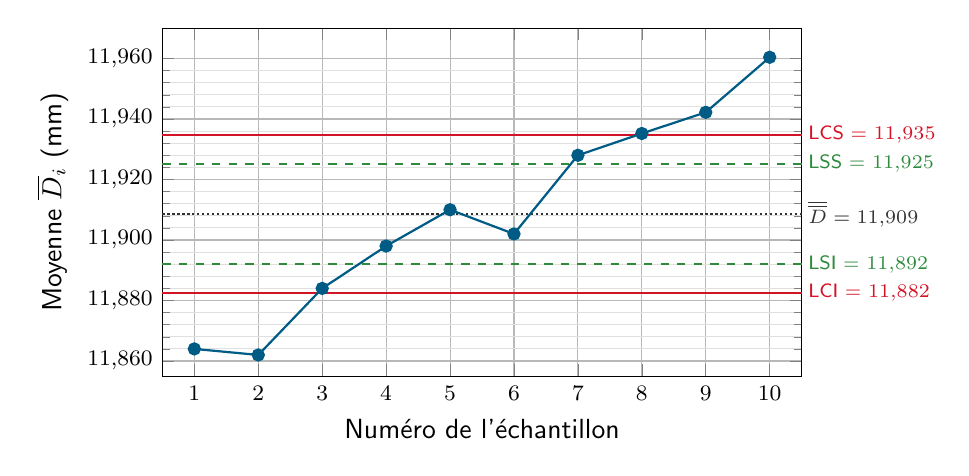
\begin{tikzpicture}
\begin{axis}[ctl, width=0.80\linewidth, clip=false, height=6.0cm, ymin=11.855, ymax=11.97, ytick={11.86,11.88,11.90,11.92,11.94,11.96}, ylabel={Moyenne $\Dbar_i$ (mm)}, yticklabel style={/pgf/number format/precision=3}]
\addplot[uimmred, thick] coordinates {(0.5,11.93472) (10.5,11.93472)} node[pos=1, anchor=west, font=\scriptsize, text=uimmred, inner sep=2pt] {LCS = $11{,}935$};
\addplot[uimmred, thick] coordinates {(0.5,11.88244) (10.5,11.88244)} node[pos=1, anchor=west, font=\scriptsize, text=uimmred, inner sep=2pt] {LCI = $11{,}882$};
\addplot[ctlgreen, thick, dashed] coordinates {(0.5,11.92516) (10.5,11.92516)} node[pos=1, anchor=west, font=\scriptsize, text=ctlgreen, inner sep=2pt] {LSS = $11{,}925$};
\addplot[ctlgreen, thick, dashed] coordinates {(0.5,11.89200) (10.5,11.89200)} node[pos=1, anchor=west, font=\scriptsize, text=ctlgreen, inner sep=2pt] {LSI = $11{,}892$};
\addplot[uimmgray, thick, densely dotted] coordinates {(0.5,11.90858) (10.5,11.90858)} node[pos=1, anchor=west, font=\scriptsize, text=uimmgray, inner sep=2pt] {$\Dbb = 11{,}909$};
\addplot[uimmblue, thick, mark=*, mark size=2pt] coordinates {(1,11.8640) (2,11.8620) (3,11.8840) (4,11.8980) (5,11.9100) (6,11.9020) (7,11.9280) (8,11.9352) (9,11.9422) (10,11.9604)};
\end{axis}
\end{tikzpicture}
\end{center}
\begin{center}
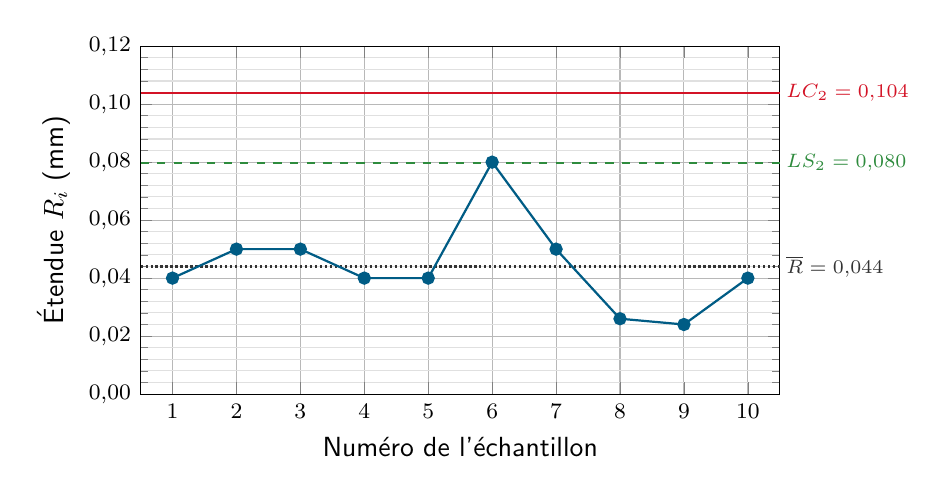
\begin{tikzpicture}
\begin{axis}[ctl, width=0.80\linewidth, clip=false, height=6.0cm, ymin=0, ymax=0.12, ytick={0,0.02,0.04,0.06,0.08,0.10,0.12}, ylabel={Étendue $R_i$ (mm)}, yticklabel style={/pgf/number format/precision=2}]
\addplot[uimmred, thick] coordinates {(0.5,0.10384) (10.5,0.10384)} node[pos=1, anchor=west, font=\scriptsize, text=uimmred, inner sep=2pt] {$LC_2 = 0{,}104$};
\addplot[ctlgreen, thick, dashed] coordinates {(0.5,0.07964) (10.5,0.07964)} node[pos=1, anchor=west, font=\scriptsize, text=ctlgreen, inner sep=2pt] {$LS_2 = 0{,}080$};
\addplot[uimmgray, thick, densely dotted] coordinates {(0.5,0.04400) (10.5,0.04400)} node[pos=1, anchor=west, font=\scriptsize, text=uimmgray, inner sep=2pt] {$\Rbar = 0{,}044$};
\addplot[uimmblue, thick, mark=*, mark size=2pt] coordinates {(1,0.040) (2,0.050) (3,0.050) (4,0.040) (5,0.040) (6,0.080) (7,0.050) (8,0.026) (9,0.024) (10,0.040)};
\end{axis}
\end{tikzpicture}
\end{center}
\piege{oublier la ligne centrale~; tracer les limites de la carte des moyennes sur la carte des étendues~; échelle de l'axe vertical qui écrase les limites.}
\end{correction}

\needspace{8cm}
\begin{correction}[-- B.5]
\source{\DR{}, §2}
\textbf{Carte des moyennes.} Sous $LCI = 11{,}882$~: les échantillons $1$ ($11{,}864$) et $2$ ($11{,}862$). Au-dessus de $LCS = 11{,}935$~: les échantillons $9$ ($11{,}942$) et $10$ ($11{,}960$), et l'échantillon $8$ ($11{,}9352$) à $0{,}5$ \textmu m de la limite. Soit $5$ points hors limites de contrôle. Entre limite de surveillance et limite de contrôle~: l'échantillon $3$ ($11{,}884$, sous $LSI = 11{,}892$) et l'échantillon $7$ ($11{,}928$, au-dessus de $LSS = 11{,}925$). Les échantillons $4$, $5$ et $6$ sont dans les limites de surveillance. Tendance nette à la hausse~: $7$ hausses sur $9$ variations, pente d'environ $10{,}7$ \textmu m par échantillon.

\textbf{Carte des étendues.} Aucun point au-dessus de $LC_2 = 0{,}104$. L'échantillon $6$ ($R_6 = 0{,}080$) est à la limite de $LS_2 = 0{,}0796$. La dispersion à l'intérieur des échantillons reste stable~; c'est la \emph{moyenne} qui bouge.

\textbf{Conclusion.} Le procédé n'est pas maîtrisé~: la moyenne dérive vers le haut, de $11{,}864$ à $11{,}960$. La carte ne dit pas la cause~: usure d'outil, échauffement, correction du régleur sont des hypothèses à vérifier sur la machine. On ne peut pas se prononcer sur la capabilité tant que le procédé n'est pas stabilisé (voir D.1).
\piege{conclure «~tout est dans la tolérance donc tout va bien~» (la question est la maîtrise, pas la conformité)~; ne regarder que la carte des étendues~; ne pas voir la tendance parce qu'aucun point des échantillons $3$ à $7$ ne sort des limites de contrôle.}
\end{correction}

\needspace{9cm}
\begin{correction}[-- B.6]
\source{\LD{}, §3.1 Définition p.~7 et §3.4 p.~8 ($P(X \geq 1) = 1 - P(X = 0)$)~; \LN{}, §3.2 p.~6}
\begin{enumerate}
  \item Par construction, $0{,}001$ en haut et $0{,}001$ en bas, soit $0{,}002$ au total.
  \item Les $10$ échantillons sont indépendants, chacun sort des limites avec la probabilité $0{,}002$~: $X \sim \mathcal{B}(10\,;0{,}002)$.
  \[
  P(X \geq 1) = 1 - P(X = 0) = 1 - 0{,}998^{10} \approx 0{,}0198.
  \]
  \item Jeu de référence~: $5$ moyennes hors limites de contrôle. Avoir \emph{au moins un} point hors limites arrive $2\,\%$ du temps~; en avoir $4$ ou plus est quasi impossible ($P(X \geq 4) \approx 3{,}3 \times 10^{-9}$). L'écart-type des $10$ moyennes vaut $33{,}0$ \textmu m, soit $3{,}9$ fois $\sigma_{\Dbar} = 8{,}5$ \textmu m. Les moyennes varient bien plus qu'un procédé stable ne le permet~: il y a une cause identifiable, ce n'est pas le hasard.
\end{enumerate}
\xlf{\texttt{=1-LOI.BINOMIALE.N(0;10;0,002;VRAI)}~; \texttt{=ECARTYPE.STANDARD(G2:G11)}.}
\piege{répondre $0{,}002 \times 10 = 0{,}02$ (valeur voisine, mais sans la loi binomiale)~; calculer $P(X = 1)$ au lieu de $P(X \geq 1)$~; comparer l'écart-type des moyennes à $\sigma$ au lieu de $\sigma_{\Dbar}$.}
\end{correction}

\needspace{8cm}
\begin{correction}[-- B.7 \textit{(pour aller plus loin)}]
\source{\LN{}, §3.2 p.~6~; \LD{}, §3.4 p.~8}
\begin{enumerate}
  \item Après le décalage, $\Dbar \sim \mathcal{N}(\mu + \sigma\,;\sigma_{\Dbar})$. La probabilité de dépasser $LCS = \mu + z_c\,\sigma_{\Dbar}$ ne dépend pas des données~:
  \[
  P(\Dbar > LCS) = P\!\left(Z > z_c - \sqrt{5}\right) = P(Z > 0{,}8541) \approx 0{,}1965.
  \]
  \item Soit $Y$ le nombre d'alarmes sur $5$ échantillons~: $Y \sim \mathcal{B}(5\,;0{,}1965)$ et $P(Y \geq 1) = 1 - (1 - 0{,}1965)^{5} \approx 0{,}665$.
\end{enumerate}
Une dérive de $1\sigma$ n'est détectée par la limite de contrôle qu'une fois sur cinq à l'échantillon suivant, et seulement deux fois sur trois sur $5$ échantillons. La limite de surveillance réagit plus tôt~: $P(\Dbar > LSS) \approx 0{,}61$. Pour un décalage de $2\sigma$, la probabilité de dépasser $LCS$ monte à $0{,}92$. C'est la raison d'être des limites de surveillance.
\xlf{\texttt{=1-LOI.NORMALE.N(LCS;D\_barre+sigma;sigma\_X;VRAI)}.}
\piege{garder la loi centrée sur $\mu$ après le décalage.}
\end{correction}

% ============================================================
\needspace{8cm}
\section{Partie C -- Capabilité du procédé}

\needspace{5cm}
\begin{correction}[-- C.1]
\source{\LN{}, §3.2 Calcul d'une probabilité p.~6}
$D \sim \mathcal{N}(11{,}9086\,;0{,}0189)$.
\[
\begin{gathered}
P(D < 11{,}85) = \texttt{LOI.NORMALE.N(11,85\,;\,}\mu\texttt{\,;\,}\sigma\texttt{\,;\,VRAI)} \approx 9{,}8 \times 10^{-4} = 978 \text{ ppm},\\
P(D > 12{,}00) = 1 - \texttt{LOI.NORMALE.N(12\,;\,}\mu\texttt{\,;\,}\sigma\texttt{\,;\,VRAI)} \approx 0{,}7 \text{ ppm}.
\end{gathered}
\]
avec $\mu = 11{,}9086$ et $\sigma = 0{,}0189$.
Soit environ $1$ pièce sur $1\,000$ sous $T_i$, et pratiquement aucune au-dessus de $T_s$.
\piege{oublier le «~$1 -$~» pour l'aire à droite~; exprimer $9{,}8 \times 10^{-4}$ en pourcentage sans conversion.}
\end{correction}

\needspace{9cm}
\begin{correction}[-- C.2]
\source{\DR{}, §3}
\begin{enumerate}
  \item $IT = 12{,}00 - 11{,}85 = 0{,}15$ mm.
  \[
  C_p = \frac{0{,}15}{6 \times 0{,}0189166} \approx 1{,}32, \quad
  \frac{T_s - \mu}{3\sigma} = \frac{0{,}0914}{0{,}05675} \approx 1{,}61, \quad \frac{\mu - T_i}{3\sigma} = \frac{0{,}0586}{0{,}05675} \approx 1{,}03.
  \]
  $C_{pk} = \min(1{,}61\,;1{,}03) = 1{,}03$.
  \item $1 \leq 1{,}03 < 1{,}33$ : \textbf{minimum acceptable, il faut améliorer le procédé}.
  \item $C_p$ ne regarde que la dispersion, $C_{pk}$ ajoute le centrage. Le milieu de la tolérance est $11{,}925$ et $\mu = 11{,}9086$~: le procédé est décentré de $16$ \textmu m vers la borne basse. Centré, il aurait $C_{pk} = C_p = 1{,}32$~: c'est encore «~minimum acceptable~». Le centrage seul ne suffit donc pas, il faut aussi réduire la dispersion.
\end{enumerate}
\piege{prendre le maximum au lieu du minimum~; calculer $C_p$ avec $\sigma$ au lieu de $6\sigma$~; conclure «~capable~» sans regarder le centrage.}
\end{correction}

\needspace{8cm}
\begin{correction}[-- C.3]
\source{\LN{}, §2.3 p.~5 et §3.2 p.~6~; \DR{}, §3}
\begin{center}
\renewcommand{\arraystretch}{1.3}
\begin{tabular}{|l|c|c|c|c|}\hline
$C_{pk}$ & $1$ & $1{,}33$ & $1{,}67$ & $2$ \\ \hline
$z = 3\,C_{pk}$ & $3$ & $3{,}99$ & $5{,}01$ & $6$ \\ \hline
$P(Z > z)$ en ppm & $1\,350$ & $33{,}0$ & $0{,}27$ & $0{,}001$ \\ \hline
\end{tabular}
\end{center}
$C_{pk} = 1{,}33$ correspond à $z \approx 4$, soit environ $33$ ppm du côté critique~: c'est le seuil de «~procédé capable~» du dossier.

\smallskip
\textbf{Inverse.} $P(Z > z) \leq 10^{-4} \iff P(Z \leq z) \geq 0{,}9999$, donc $z \geq \texttt{LOI.NORMALE.STANDARD.INVERSE.N(0,9999)} \approx 3{,}719$ et $C_{pk} \geq 3{,}719/3 = 1{,}2397$. On arrondit par excès~: $C_{pk} \geq 1{,}24$. Avec $1{,}23$, $z = 3{,}69$ et $P \approx 1{,}12 \times 10^{-4}$~: l'exigence n'est pas respectée. Le $C_{pk}$ du procédé ($1{,}03$) est en dessous.
\xlf{\texttt{=ARRONDI.SUP(3,719/3;2)}.}
\piege{arrondir à $1{,}23$ (arrondi «~au plus proche~»)~; saisir $10^{-4}$ comme aire à gauche.}
\end{correction}

\needspace{8cm}
\begin{correction}[-- C.4]
\source{\LN{}, §4.2 Retrouver un paramètre $\mu$ ou $\sigma$ p.~8~; §2.3 p.~5}
Exigence $P(D < T_i) \leq 10^{-4}$~: $\dfrac{T_i - \mu}{\sigma} \leq -3{,}719$, soit $\mu \geq T_i + 3{,}719\,\sigma$.
\begin{enumerate}
  \item $\mu \geq 11{,}85 + 3{,}719 \times 0{,}0189166 = 11{,}92035$. Par excès au micromètre~: $\mu_{\min} = 11{,}921$.
  \item $P(D > T_s) \leq 10^{-4}$ donne $\mu \leq 12{,}00 - 0{,}07035 = 11{,}92965$. Par défaut~: $\mu_{\max} = 11{,}929$.
  \item La fenêtre est $[11{,}921\,;11{,}929]$, de largeur $8$ \textmu m après arrondis ($9{,}3$ \textmu m avant)~: c'est $IT$ moins $2 \times 3{,}719\,\sigma \approx 140{,}7$ \textmu m. Le réglage actuel $11{,}9086$ est \textbf{hors fenêtre}, à $12$ \textmu m sous $\mu_{\min}$. Même si on le corrigeait, une fenêtre de $8$ \textmu m est trop étroite pour un réglage à la main~: $\sigma$ est trop grand.
\end{enumerate}
\xlf{\texttt{=ARRONDI.SUP(Ti+z*sigma;3)} et \texttt{=ARRONDI.INF(Ts-z*sigma;3)}.}
\piege{arrondir $\mu_{\min}$ à $11{,}920$ ou $\mu_{\max}$ à $11{,}930$ (sens contraire à l'exigence)~; ne traiter qu'un côté~; conclure «~dans la fenêtre~» parce que $C_{pk} > 1$.}
\end{correction}

\needspace{6cm}
\begin{correction}[-- C.5]
\source{\LN{}, §4.2 p.~8}
$50$ ppm au total, procédé centré~: $25$ ppm de chaque côté. Il faut $P(D > 12{,}00) \leq 25 \times 10^{-6}$ avec $\mu = 11{,}925$~:
\[
\begin{gathered}
z = \texttt{LOI.NORMALE.STANDARD.INVERSE.N}(1 - 25 \times 10^{-6}) \approx 4{,}0556,\\
\frac{12{,}00 - 11{,}925}{\sigma} \geq z \iff \sigma \leq \frac{0{,}075}{4{,}0556} = 18{,}49 \text{ \textmu m}.
\end{gathered}
\]
Par défaut au dixième de \textmu m~: $\sigma_{\max} = 18{,}4$ \textmu m. Vérification~: avec $18{,}4$, on obtient $45{,}8$ ppm~; avec $18{,}5$, $50{,}3$ ppm (exigence dépassée). Le procédé actuel a $\sigma = 18{,}9$ \textmu m, au-dessus de $\sigma_{\max}$~: même \emph{parfaitement centré}, il donnerait environ $73$ ppm, donc l'exigence du client n'est pas tenue. Résultat cohérent avec $C_p = 1{,}32 < 1{,}33$.
\piege{prendre $50$ ppm de chaque côté~; arrondir à $18{,}5$~; ne pas comparer à $\sigma$.}
\end{correction}

% ============================================================
\needspace{9cm}
\section{Partie D -- Synthèse et décision}

\needspace{7cm}
\begin{correction}[-- D.1]
\source{\DR{}, §1 et §3~; \LN{}, §3.1 p.~6}
\begin{enumerate}
  \item $s = 35{,}9$ \textmu m sur les $50$ mesures, soit environ $1{,}9$ fois $\sigma = 18{,}9$ \textmu m.
  \item $C_p' = \dfrac{0{,}15}{6 \times 0{,}035855} \approx 0{,}70$ et $C_{pk}' = \min\!\left(\dfrac{0{,}0914}{3 \times 0{,}035855}\,;\dfrac{0{,}0586}{3 \times 0{,}035855}\right) = \min(0{,}85\,;0{,}54) \approx 0{,}54$. Avec $C_{pk}' < 1$, le procédé \textbf{n'est pas capable} de tenir toute la production dans la tolérance sur la durée. (On note souvent ces indices «~long terme~» $P_p$ et $P_{pk}$.)
  \item $\sigma = \Rbar/d_n$ mesure la dispersion \emph{à l'intérieur} des échantillons (court terme). $s$ mélange cette dispersion et le déplacement des moyennes d'un échantillon à l'autre, visible sur les cartes. L'écart entre $s$ et $\sigma$ est la signature de la dérive. La droite de Henry n'avait pas alerté parce qu'elle regarde l'ensemble des valeurs sans leur ordre dans le temps~: une dérive régulière étale les valeurs et donne une distribution d'allure normale.
\end{enumerate}
\xlf{\texttt{=ECARTYPE.STANDARD(Mesures!B2:F11)}.}
\piege{retenir seulement $C_{pk} = 1{,}03$ de la partie C~; ne pas relier l'écart à la dérive~; conclure que la droite de Henry «~s'est trompée~».}
\end{correction}

\needspace{7cm}
\begin{correction}[-- D.2]
\source{\LN{}, §3.2 p.~6 et §3.3 p.~7}
Avec $\sigma = 0{,}0189166$ mm~:
\[
\begin{gathered}
\text{éch. 1 } (\mu = 11{,}864)\,:\ P(D < 11{,}85) = \texttt{LOI.NORMALE.N(11,85\,;\,}\mu\texttt{\,;\,}\sigma\texttt{\,;\,VRAI)} \approx 0{,}230,\\
\text{éch. 10 } (\mu = 11{,}9604)\,:\ P(D > 12{,}00) = 1 - \texttt{LOI.NORMALE.N(12\,;\,}\mu\texttt{\,;\,}\sigma\texttt{\,;\,VRAI)} \approx 0{,}018.
\end{gathered}
\]
Au départ, le modèle prévoit $23\,\%$ de pièces sous $T_i$~; à la fin, $1{,}8\,\%$ au-dessus de $T_s$. La prévision de la question C.1 était de $978$ ppm, soit $0{,}1\,\%$.

\textbf{Réalité.} Parmi les $50$ pièces, $2$ sont hors tolérance (deux mesures à $11{,}84$, dans les échantillons $1$ et $2$), soit $4\,\%$ ou $40\,000$ ppm. C'est environ $40$ fois la prévision du $C_{pk}$ global. Le $C_{pk}$ de $1{,}03$ est une moyenne qui masque la situation de départ~: il prédit $978$ ppm en supposant que $\mu$ est fixe, alors qu'il bouge. L'échantillon $1$ contient bien $1$ pièce sur $5$ sous $T_i$ ($20\,\%$), ce qui est cohérent avec les $23\,\%$ prévus échantillon par échantillon.
\piege{conclure que le modèle est faux parce qu'aucune pièce n'est au-dessus de $T_s$ dans l'échantillon $10$ (l'échantillon est trop petit pour le voir)~; compter les deux mesures à $11{,}85$ comme hors tolérance (la borne est incluse).}
\end{correction}

\needspace{7cm}
\begin{correction}[-- D.3]
\source{\LN{}, §4.2 p.~8~; §3.2 p.~6}
Pente de la droite d'évolution des moyennes~: $10{,}7$ \textmu m par échantillon. La dernière moyenne est $11{,}9604$~; marge restante jusqu'à $T_s$~: $12{,}000 - 11{,}9604 = 0{,}0396$ mm. Durée~: $39{,}6/10{,}7 \approx 3{,}7$, soit environ $4$ échantillons. C'est un ordre de grandeur tiré de $10$ points, pas une prévision. Quand la moyenne atteint $T_s$, la moitié des pièces dépasse la tolérance.

\textbf{Actions possibles.} Régleur~: recentrer vers le milieu de la tolérance ($11{,}925$) avec le correcteur d'outil, puis corriger dès qu'un point sort des limites de surveillance. Technicien méthodes~: rechercher la cause de la dérive (usure de l'outil, échauffement de la broche ou de la pièce, correction manuelle répétée), réduire la dispersion (la fenêtre de la question C.4 est trop étroite) et resserrer l'intervalle de prélèvement. Après stabilisation, refaire l'étude avec $100$ à $200$ mesures pour calculer $C_p$ et $C_{pk}$ fiables.
\xlf{\texttt{=PENTE(Mesures!G2:G11;Mesures!A2:A11)}.}
\piege{proposer une cause comme un fait établi~; proposer d'élargir la tolérance~; recentrer sans réduire la dispersion alors que $C_p < 1{,}33$.}
\end{correction}

\end{document}
